\documentclass[11pt,a4paper]{article}

\usepackage[margin=1cm]{geometry}
\usepackage{amssymb}
\usepackage{graphicx}  % For images
\usepackage{multicol}  % For columns
\usepackage{wrapfig}   % For wrapping text around images
\usepackage{tikz}
\usepackage{pgf}
\usepackage{multirow}
\usepackage{enumitem}
\usepackage{lmodern}
\usepackage{changepage}
\usepackage{ragged2e}
\usepackage{tcolorbox}
\usepackage{xcolor}
\usepackage{fontawesome}

\usepackage[T1]{fontenc}
\usepackage{inter}

\pagenumbering{gobble}
\raggedright
\begin{document}

% COMMANDS
\newcommand{\header}[1]{%
    \vspace{-0.3em}
    {\tiny\section*{\small{#1}}\vspace{-2.5em}}
    \hrulefill\vspace{0.7em}
}

\newcommand{\contact}{
    \begin{center}
    \faGlobe\ codyj.io% 
    \hspace{1em}\textbar\hspace{1em}%
    \faEnvelope\ codywj777@gmail.com% 
    \hspace{1em}\textbar\hspace{1em}%
    \faPhone\ (604) 802-6801% 
    \hspace{1em}\textbar\hspace{1em}%
    \faGithub\ github.com/cody-j%
    \end{center}
}

\newcommand{\pill}[2][gray!10]{%
    % \tcbox[nobeforeafter,colback=#1,colframe=#1,left=4pt,right=4pt,top=2pt,bottom=2pt,tcbox raise base]{\textbf{#2}}
    \tcbox[
        height=0.4cm,
        nobeforeafter,
        valign=center,
        width=fit,
        colback=#1,
        colframe=#1,
        left=2pt,
        right=2pt,
        boxrule=0pt,
    ]{\tiny\color{gray!10}\textbf{#2}}
}

\newcommand{\experience}[4]{%  % Title, Company, Date, Highlights
    \textbf{\normalsize #1} {\small\textbar{}} \raisebox{0ex}{\small{#2}} \hfill \raisebox{0.1ex}{\small\textbf{#3}}%
    \vspace{0.4em}%
    \begin{adjustwidth}{0.3cm}{0.3cm}%
        \begin{itemize}[leftmargin=*, nosep]%
            #4
        \end{itemize}%
    \end{adjustwidth}%
    \vspace{1em}%
}
% END COMMANDS

% HEADER
\begin{minipage}{0.7\textwidth}
    {\huge \textbf{Cody Johnson}}\\[0.5em]
    {\Large Software Engineer}\\[0.3em]
    {Vancouver, BC}
\end{minipage}%
\begin{minipage}{0.3\textwidth}
    \begin{flushright}
        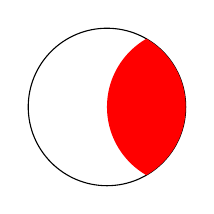
\begin{tikzpicture}
            \draw[clip] (0,0) circle (1cm);
            \fill[red] (1,0) circle (1cm);
          \end{tikzpicture}
    \end{flushright}
\end{minipage}

\vspace{1em}

% SUMMARY
\begin{tcolorbox}[
    colback=gray!10,    % background color
    colframe=gray!10,   % frame color (same as background for no visible frame)
    left=10pt,          % left padding
    right=10pt,         % right padding
    top=5pt,            % top padding
    bottom=5pt          % bottom padding
]
    \begin{adjustwidth}{}{}
        \vspace{0.1cm}
        \justify\normalfont
        Technical leader and full-stack engineer specializing in distributed systems and cloud architecture. Led engineering teams at high-growth startups, architected enterprise-scale data pipelines, and founded a B2B SaaS company. Consistently delivers high-impact solutions in AWS with expertise in TypeScript/Node.js ecosystems and data engineering. Track record of optimizing system performance and scaling applications from concept to production.
        \vspace{0.1cm}
    \end{adjustwidth}
\end{tcolorbox}

\contact

% Skills
\header{SKILLS}

\begin{adjustwidth}{0.3cm}{0.2cm}
    \pill[blue!70]{NODE}%
    \pill[blue!70]{PYTHON}%
\end{adjustwidth}

\vspace{1em}


\header{EXPERIENCE}

\experience{Technical Founder}{Skoookum}{May 2021 - Present}{%        
    \item Architected and implemented application infrastructure spanning AWS and Azure, including Lambda services, PostgreSQL databases, and Redis caching layer%
    \item Designed and built a Vue-based Excel Add-In to create and manage granular entities within a workbook%
    \item Integrated with Microsoft Entra and the Commercial Marketplace to handle authentication, authorization, and subscription state%
}

\experience{Lead Software Engineer}{Treez}{December 2021 - April 2024}{%
    \item Led development of our eventing system on top of Eventbridge and Kinesis, decoupling services in what had become a distributed monolith%
    \item Led development of enterprise ELT pipeline processing data from 400+ MySQL instances reducing report generation time by 90\%, enabling real-time business insights for our users%
    \item Implemented analytics platform on DBT + Quicksight reducing cogs by hundreds of thousands of dollars per year%
    \item Architected and implemented a Data Lake House on top of AWS primitives to support the analytics platform%
}

\experience{Software Engineer}{Treez}{September 2020 - December 2021}{%
    \item Orchestrated migration from EC2 to Kubernetes enabling zero-downtime deployments%
    \item Optimized critical track-and-trace queries reducing latency in one case from +10s to <300ms%
    \item Integrated track-and-trace system with delivery partners enabling millions of dollars in new business%
}

% Second Page
\newpage

% EXPERIENCE (cont'd)
\header{EXPERIENCE (cont'd)}

\experience{Software Engineer}{Electronic Arts}{January 2020 - September 2020}{%
    \item Enhanced build system to better handle a particular class of error, eliminating hundreds of lost man-hours over a week%
    \item Worked with game developers and game testers to facilitate proper output from Jenkins farm%
}

\experience{Software Engineer}{Indigo Ag}{January 2019 - December 2019}{%
    \item Agricultural intelligence platform combining satellite imagery with precision farming technology%
    \item Built React-based visualization platform connecting 100TB+ of satellite imagery data with agronomists%
    \item Developed ETL pipeline processing WKT data into vector tiles, integrated into Airflow processes%
}

\experience{Software Engineer}{Control}{January 2017 - December 2018}{%
    \item Payment data studio with cross-platform aggregation%
    \item Implemented V2 of business intelligence platform processing \$500M+ in payment data from the four major providers%
    \item Implemented auto-scaling system to handle spikes in pipeline ingestion%
}

% EDUCATION
\header{EDUCATION}

\textbf{\normalsize Mechanical Engineering} {\small\textbar{}} \raisebox{0ex}{\small{BCIT}} \hfill \raisebox{0.1ex}{\small\textbf{2009-2011}}
\vspace{0.8em}

\textbf{\normalsize Web Development} {\small\textbar{}} \raisebox{0ex}{\small{Lighthouse Labs}} \hfill \raisebox{0.1ex}{\small\textbf{2016}}
\vspace{0.8em}

\textbf{\normalsize Motorcycle Mechanics} {\small\textbar{}} \raisebox{0ex}{\small{BCIT}} \hfill \raisebox{0.1ex}{\small\textbf{2016}}
\vspace{2em}

% CERTIFICATES
\header{CERTIFICATES}

\textbf{\normalsize AWS Cloud Practitioner} {\small\textbar{}} \raisebox{0ex}{\small{Amazon}} \hfill \raisebox{0.1ex}{\small\textbf{2021}}
\vspace{2em}

% CLUBS
\header{CLUBS}

\textbf{\normalsize First Robotics Challenge} {\small\textbar{}} \raisebox{0ex}{\small{Sullivan Heights}} \hfill \raisebox{0.1ex}{\small\textbf{2008-2009}}
\vspace{2em}

\vfill

\contact

\end{document}
